\documentclass{article}
\usepackage[a4paper]{geometry}
\usepackage[utf8]{inputenc}
\usepackage{polski}
\usepackage{tabularx}
\usepackage{indentfirst}
\usepackage{multirow}
\usepackage{amssymb}
\usepackage{amsmath}
\usepackage{anysize}
\usepackage{float}
\usepackage{caption}
\usepackage{subcaption}
\usepackage{graphicx}

\usepackage{listings}
\usepackage{color}
\lstset{literate=%
{ą}{{\k{a}}}1 {ć}{{\'c}}1 {ę}{{\k{e}}}1 {ł}{{\l{}}}1 {ń}{{\'n}}1 {ó}{{\'o}}1 {ś}{{\'s}}1 {ż}{{\.z}}1 {ź}{{\'z}}1 {Ą}{{\k{A}}}1 {Ć}{{\'C}}1 {Ę}{{\k{E}}}1 {Ł}{{\L{}}}1 {Ń}{{\'N}}1 {Ó}{{\'O}}1 {Ś}{{\'S}}1 {Ż}{{\.Z}}1 {Ź}{{\'Z}}1 }

\definecolor{mygreen}{rgb}{0,0.6,0}
\definecolor{mygray}{rgb}{0.5,0.5,0.5}
\definecolor{mymauve}{rgb}{0.58,0,0.82}

\usepackage{titling}
\newcommand{\subtitle}[1]{%
	\posttitle{%
	\par\end{center}
	\begin{center}\small#1\end{center}
	\vskip0.5em}%
}

\title{Algenic -- serwis z~konkursami algorytmicznymi}
\subtitle{Akademia Górniczo-Hutnicza im. Stanisława Staszica w Krakowie\\
	Wydział Elektrotechniki, Automatyki,\\
	Informatyki i Inżynierii Biomedycznej}
\author{Kacper Tonia\and
		Sławomir Kalandyk\and
		Mateusz Ruciński}
\date{}

\begin{document}
%------------------------------------------------------------
\maketitle

%------------------------------------------------------------
\section{Wymagania projektowe}

\subsection{Dramatis personae}

Użytkownik:
\begin{itemize}
	\item Wysyła rozwiązania zadań konkursowych i~jest za~nie odpowiednio punktowany
	\item Po zakończeniu konkursu, każdy użytkownik może zobaczyć ranking
	\item Sformatowanie standardowego wyjścia programu leży po~stronie użytkownika wysyłającego rozwiązanie, np.~jeśli akceptowane rozwiązanie jest postaci ,,\texttt{x~y}'', gdzie \texttt{x}~i~\texttt{y} to~liczby, to~użytkownik powinien zadbać, aby wyjście jego programu przyjmowało taką formę
	\item Rozwiązanie zadania powinno być wysyłane przez użytkownika jako plik z~kodem
\end{itemize}

Organizator konkursów:
\begin{itemize}
	\item Można założyć, że~jest tylko jeden organizator konkursów
	\item Tylko organizator konkursów może tworzyć nowe konkursy i~dodawać do~nich zadania
	\item Dodaje odpowiednio sformatowane przypadki testowe do~zadań, względem których jest porównywane standardowe wyjście programu użytkownika
	\item Ustala ilość punktów otrzymanych przez użytkownika za~rozwiązanie (w~pełni lub częściowe) zadania
\end{itemize}

Serwer/administrator:
\begin{itemize}
	\item Zleca kompilację kodu użytkownika, dokonuje oceny i~zwraca odpowiedni feedback użytkownikowi
	\item Przechowuje standardowe wyjście błędu i~loguje je, w~razie potrzeby wyświetla użytkownikowi
	\item Przechowuje historie przesłanych rozwiązań
	\item Dba o~podstawowe kwestie bezpieczeństwa -- nie przechowuje haseł jako plaintext, uniemożliwia SQL injection
\end{itemize}

Pozostałe wymagania:
\begin{itemize}
	\item System antyplagiatowy nie jest konieczny
	\item Kwestia prezentacji projektu - czy na serwerze zewnętrznym (dostęp przez internet), czy na własnej maszynie, wybór jest dowolny
\end{itemize}

%------------------------------------------------------------
\newpage
\section{Przypadki użycia}


\begin{figure}[H]
	\centering
	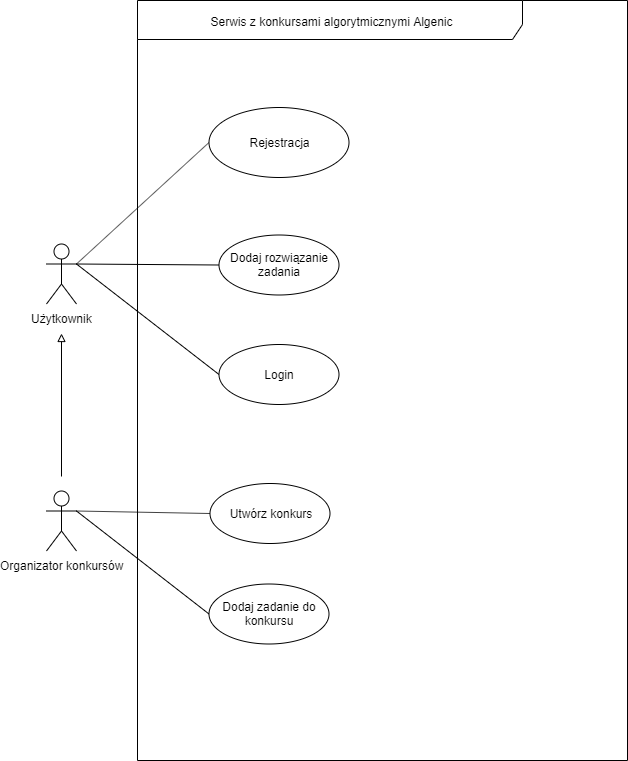
\includegraphics[width=.6\linewidth]{useCases.png}
	\caption{Diagram przypadków użycia}
\end{figure}

\subsection{Dodanie rozwiązania zadania}

\textbf{Aktorzy:} Użytkownik

\textbf{Zakres:} Serwis z konkursami algorytmicznymi Algenic

\textbf{Cel (story):} Dodanie rozwiązania do zadania

\textbf{Warunki początkowe:} Użytkownik jest uczestnikiem aktywnego konkursu, konkurs posiada przynajmniej jedno (nierozwiązane przez użytkownika) zadanie

\textbf{Warunek końcowy dla powodzenia:} Zadanie zostaje rozwiązane, użytkownik zostaje powiadomiony o poprawnym wykonaniu zadania

\textbf{Warunek końcowy dla niepowodzenia:} Zadanie nie zostaje rozwiązane, użytkownik zostaje powiadomiony o niepowodzeniu oraz rodzaju błędu

\textbf{Zdarzenie wyzwalające (trigger):} Użytkownik wybiera zadanie z konkursu, którego jest uczestnikiem i wybiera funkcję dodania rozwiązania zadania

\textbf{Scenariusz główny:}
\begin{enumerate}
	\item Użytkownik wybiera konkurs
	\item Użytkownik wybiera zadanie
	\item Serwis wyświetla treść zadania i udostępnia możliwość wrzucenia rozwiązania w postaci pliku z rozwiązaniem
	\item Użytkownik wrzuca plik z rozwiązaniem zadania
	\item Serwis wielokrotnie kompiluje plik z rozwiązaniem z różnymi danymi wejściowymi
	\item Serwis porównuje dane wyjściowe kompilacji z poprawnymi rozwiązaniami zadania
	\item Serwis zapisuje plik oraz wynik kompilacji (sukces/treść błędu) w historii
	\item Serwis zwraca wiadomość o poprawności wykonania zadania. Koniec przypadku użycia.
\end{enumerate}

\textbf{Rozszerzenia scenariusza głównego:}
\begin{itemize}
	\item[5a.] Kompilacja nie powiodła się
	\item[5a1.] Serwis zwraca wiadomość o niepowodzeniu kompilacji wraz z treścią błędu. Koniec przypadku użycia
	\item[6a.] Dane wyjściowe kompilacji nie stanowią poprawnego rozwiązania zadania
	\item[6a1.] Serwis zwraca wiadomość o niepoprawnym rozwiązaniu zadania. Koniec przypadku użycia.
\end{itemize}

\newpage
\subsection{Utwórz konkurs}

\textbf{Aktorzy:} Organizator konkursów

\textbf{Zakres:} Serwis z konkursami algorytmicznymi Algenic

\textbf{Cel (story):} Organizator konkursów chce utworzyć nowy konkurs

\textbf{Warunki początkowe:} Organizator konkursów jest zalogowany

\textbf{Warunek końcowy dla powodzenia:} Konkurs został utworzony

\textbf{Warunek końcowy dla niepowodzenia:} Konkurs nie został utworzony

\textbf{Zdarzenie wyzwalające (trigger):} Organizator konkursów wybiera opcję utworzenia nowego konkursu

\textbf{Scenariusz główny:}
\begin{enumerate}
	\item Organizator konkursów wybiera funkcję utworzenia nowego konkursu
	\item Serwis wyświetla formularz utworzenia nowego konkursu
	\item Organizator konkursu wprowadza nazwę konkursu
	\item Zostaje utworzony nowy konkurs w stanie ,,nierozpoczęty''. Koniec przypadku użycia.
\end{enumerate}


\subsection{Dodaj zadanie do istniejącego konkursu}

\textbf{Aktorzy:} Organizator konkursów  

\textbf{Zakres:} Serwis z konkursami algorytmicznymi Algenic  

\textbf{Cel (story):} Organizator konkursów chce dodać zadanie do konkursu  

\textbf{Warunki początkowe:} Organizator konkursów ma możliwość dokonywania zmian w konkursie w stanie "nierozpoczęty"  

\textbf{Warunek końcowy dla powodzenia:} Zadanie zostało dodane do konkursu  

\textbf{Warunek końcowy dla niepowodzenia:} Zadanie nie zostało dodane do konkursu, zostaje wyświetlony komunikat o niepowodzeniu  

\textbf{Zdarzenie wyzwalające (trigger):} Organizator konkursów wybiera konkurs w stanie "nierozpoczęty" i wybiera opcję dodania zadania 
do konkursu
\textbf{Scenariusz główny:}
\begin{enumerate}
	\item Organizator konkursów wybiera konkurs w stanie "nierozpoczęty"
	\item Organizator konkursów wybiera funkcję dodania zadania do konkursu
	\item Serwis wyświetla formularz do dodania nowego zadania
	\item Organizator konkursów wypełnia formularz
	\item Nowe zadanie zostaje dodane do konkursu. Koniec przypadku użycia.
\end{enumerate}

\textbf{Rozszerzenia scenariusza głównego:}
\begin{itemize}
	\item[4a.] Formularz został wypełniony nieprawidłowo  
	\item[4a1.] Zostaje wyświetlony komunikat o niepowodzeniu. Koniec przypadku użycia.
\end{itemize}

\newpage
\subsection{Rejestracja}

\textbf{Aktorzy:} Użytkownik

\textbf{Zakres:} Serwis z konkursami algorytmicznymi Algenic

\textbf{Cel (story):} Użytkownik chce się zarejestrować

\textbf{Warunki początkowe:} Użytkownik nie jest zarejestrowany

\textbf{Warunek końcowy dla powodzenia:} Użytkownik zostaje zarejestrowany

\textbf{Warunek końcowy dla niepowodzenia:} Użytkownik nie zostaje zarejestrowany, zostaje wyświetlony komunikat o niepowodzeniu

\textbf{Zdarzenie wyzwalające (trigger):} Użytkownik wybiera funkcję rejestracji

\textbf{Scenariusz główny:}
\begin{enumerate}
	\item Serwis wyświetla formularz rejestracji
	\item Użytkownik wprowadza email oraz hasło (email służy jako login)
	\item Następuje weryfikacja wprowadzonych danych po stronie serwisu
	\item Użytkownik zostaje zarejestrowany. Koniec przypadku użycia.
\end{enumerate}

\textbf{Rozszerzenia scenariusza głównego:}
\begin{itemize}
	\item[3a.] Weryfikacja zakończona niepowodzeniem (email już istnieje w bazie, lub hasło nie spełnia warunków)
	\item[3a1.] Zostaje wyświetlony komunikat o niepowodzeniu. Koniec przypadku użycia.
\end{itemize}

% \newpage
\subsection{Logowanie}

\textbf{Aktorzy:} Użytkownik

\textbf{Zakres:} Serwis z konkursami algorytmicznymi Algenic

\textbf{Cel (story):} Użytkownik chce się zalogować

\textbf{Warunki początkowe:} Użytkownik jest w stanie niezalogowanym

\textbf{Warunek końcowy dla powodzenia:} Użytkownik zmienia stan na zalogowany

\textbf{Warunek końcowy dla niepowodzenia:} Użytkownik nie zmienia stanu na zalogowany, zostaje wyświetlony komunikat o błędzie

\textbf{Zdarzenie wyzwalające (trigger):} Użytkownik wybiera funkcję zalogowania

\textbf{Scenariusz główny:}
\begin{enumerate}
	\item Serwis wyświetla formularz do logowania
	\item Użytkownik wprowadza login oraz hasło
	\item Następuje autentykacja danych po stronie serwisu
	\item Stan użytkownika zostaje zmieniony na zalogowany. Koniec przypadku użycia.
\end{enumerate}

\textbf{Rozszerzenia scenariusza głównego:}
\begin{itemize}
	\item[3a.] Autentykacja nie powiodła się
	\item[3a1.] Serwis wyświetla komunikat o błędzie. Koniec przypadku użycia.
\end{itemize}

%------------------------------------------------------------
\newpage
\section{Architektura}

\begin{figure}[H]
	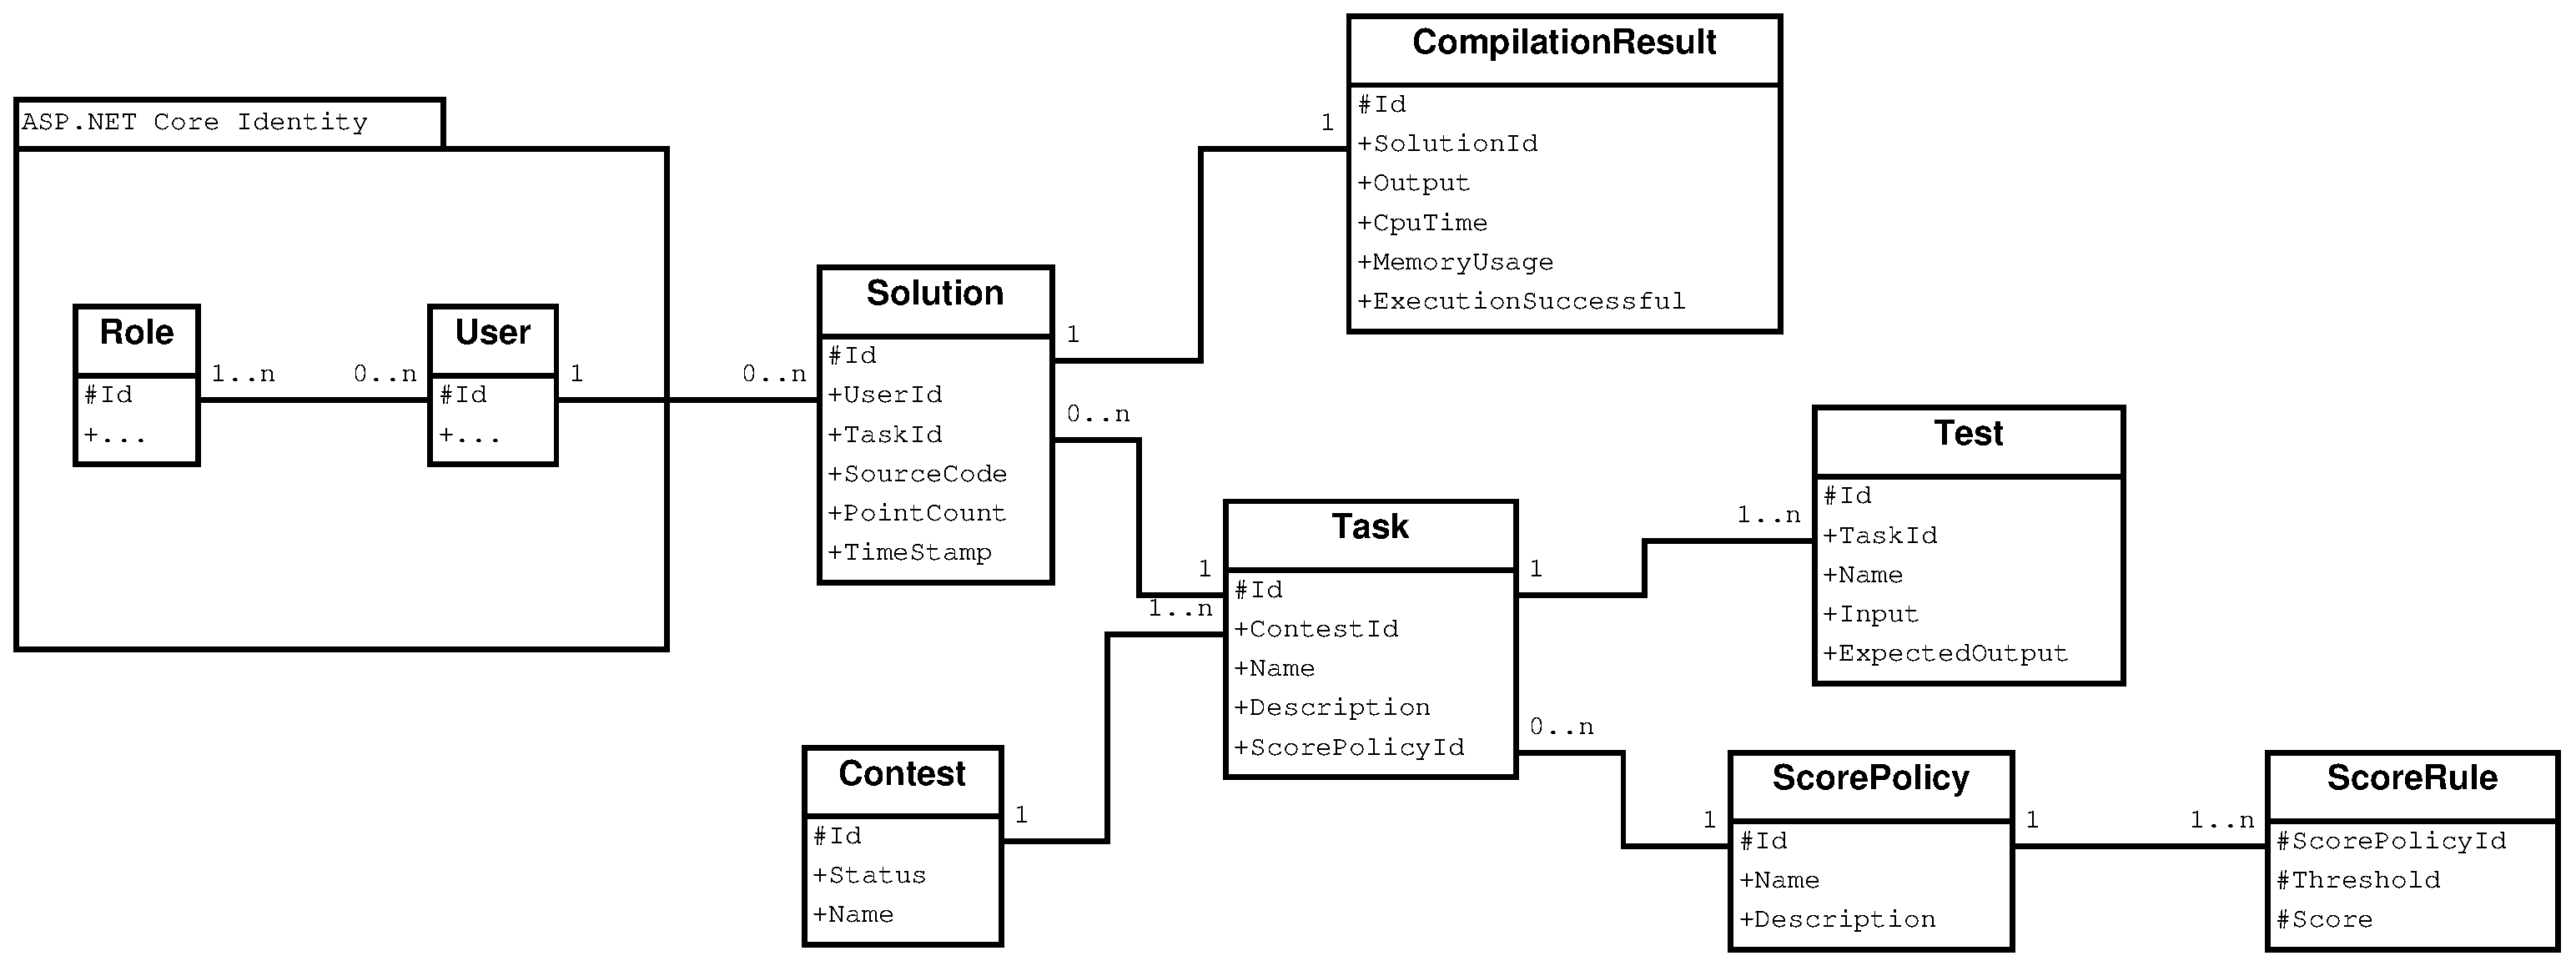
\includegraphics[width=\linewidth]{entityDiagram.eps}
	\caption{Diagram bazy danych}
\end{figure}

\begin{figure}[H]
	\centering
	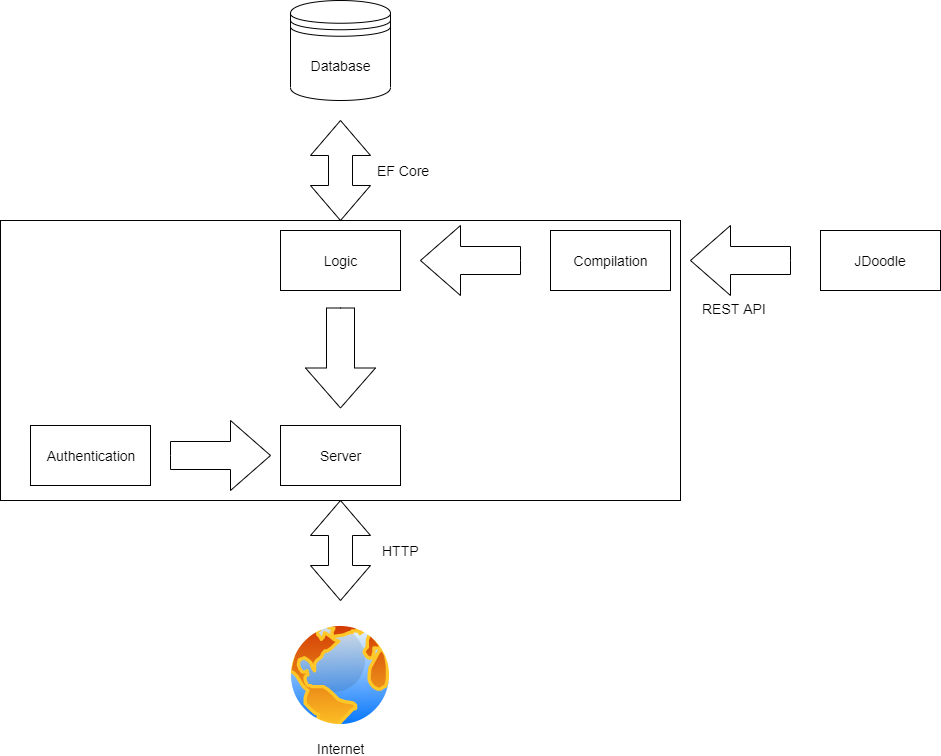
\includegraphics[width=\linewidth]{projectModules.png}
	\caption{Diagram modułów}
\end{figure}

\subsection{Opis interfejsów}
Do połączenia z~bazą danych zostanie wykorzystany \textbf{Entity Framework Core}, służący do~mapowania obiektowo-relacyjnego. Pozwala on~na~wygenerowanie klas będących podstawą komunikacji z~bazą danych. Tworzenie zapytań do~bazy danych jest w~nim możliwe przy użyciu zapytań LINQ (Language Integrated Query).

Kompilacja plików będzie się odbywała za~pomocą JDoodle. Udostępnia on~API pozwalające na~zdalną kompilację. Odbywa się to~poprzez przesłanie zapytania POST w~formacie JSON na~konkretny, stały adres. W~zapytaniu powinny znajdować się m.in.~język oraz kod źródłowy programu. W~zamian, API zwraca wynik kompilacji.

Do utworzenia GUI posłuży framework ASP.NET Core wykorzystujący Razor Pages. Razor Pages bazuje na wzorcu architektonicznym MVVM.

%------------------------------------------------------------
\section{Technologia i~narzędzia}

\textbf{Język programowania:} C\#

\textbf{Framework:} ASP.NET~Core~2.2

\textbf{System kontroli wersji:} Git

\textbf{Platforma:} GitHub

\textbf{Serwis do testów automatycznych:} Travis CI

\textbf{Zdalna kompilacja:} JDoodle

Projekt został oparty o~framework ASP.NET~Core ze~względu na~jego popularność, wieloplatformowość i~fakt bycia oprogramowiem typu open source. Zrezygnowaliśmy z~sięgnięcia po~najnowszą wersję frameworka,~3.0, na~rzecz bardziej dojrzałej i~potencjalnie stabilniejszej wersji~2.2.

Rozważyliśmy wykorzystanie usługi Azure, co~pozwoliłoby na~skupienie większości aspektów pracy nad~programem w~jednym miejscu (począwszy od~przechowywania plików projektu, poprzez zarządzanie bazą danych projektu, skończywszy na~automatycznym testowaniu zmian i~wdrażaniu aktualnej wersji aplikacji w~chmurze Azure). Stosunkowo długie czasy testowania i~wdrażania w~chmurze, a~także względnie niewielka złożoność naszego projektu sprawiły, że~zdecydowaliśmy się na~uruchamianie~i~testowanie aplikacji lokalnie, wraz z~lokalną bazą danych w~technologii SQL~Server.

Ostatecznie wybraliśmy platformę GitHub m.in.~ze~względu na~wbudowane narzędzia do~zarządzania projektem, takie jak tablica zadań, które ułatwią systematyzację zadań związanym z~etapem implementacji i~przydzielanie owych zadań członkom zespołu. Jako element praktyki \emph{Continuous Integration}, zmiany dodawane do~głównego repozytorium są~automatycznie testowane na~platformie \textbf{Travis~CI}.

Na~późniejszym etapie prac nad projektem możemy ponownie rozważyć wykorzystanie Azure, chociażby w~celu uruchomienia wspólnej, trwałej bazy danych w~chmurze.

W~celu kompilowania kodów przysyłanych przez użytkowników wykorzystamy serwis \textbf{JDoodle}, oferujący REST-owe API do~zdalnej kompilacji. Kompilowanie niezaufanego kodu na~serwerze niosłoby poważne zagrożenie, o~ile nie podjęlibyśmy specjalnych środków bezpieczeństwa. Użycie istniejącej usługi jak JDoodle redukuje potencjalne problemy z~bezpieczeństwem.

W~darmowym wariancie JDoodle pozwala na~przeprowadzenie ok.~200 kompilacji dziennie. Może być to~zbyt mała wartość podczas intensywnego testowania, jednak prostota użycia i~bogata ilość dostępnych języków programowania przekonuje nas ostatecznie do~owego rozwiązania.

%------------------------------------------------------------
\section{Testy}

Testy wchodzące w~skład projektu możemy podzielić na~testy jednostkowe i~funkcjonalne. Wybranym frameworkiem testowym jest \textbf{xunit}. Do~testów funkcjonalnych dodatkowo wykorzystujemy \textbf{Selenium WebDriver} -- framework automatyzujący operacje na~przeglądarkach internetowych.

Celem testów jednostkowych jest weryfikacja działania możliwie małych, odizolowanych od~siebie elementów kodu. Mija się z~celem jednak testowanie np.~każdej metody z~osobna, gdyż wymuszałoby to~uczynienie wszystkich metod publicznymi. Zamiast tego proponujemy, aby~klasy upubliczniały absolutne minimum funkcjonalności. Ów~publiczny interfejs będziemy poddawać testom jednostkowym.

Użytkownik przeważnie nie jest jednak zainteresowany działaniem pojedynczych elementów składowych aplikacji, stąd pomysł wprowadzenia testów funkcjonalnych, które testują znaczną część aplikacji z~punktu widzenia użytkownika. W~naszym przypadku testy funkcjonalne opierają się na~realizacji szeregu zautomatyzowanych operacji w~przeglądarce internetowej i~sprawdzeniu, czy odpowiedź aplikacji spełnia nasze oczekiwania.

%------------------------------------------------------------
\section{Analiza ryzyka}


\begin{figure}[H]
	\centering
	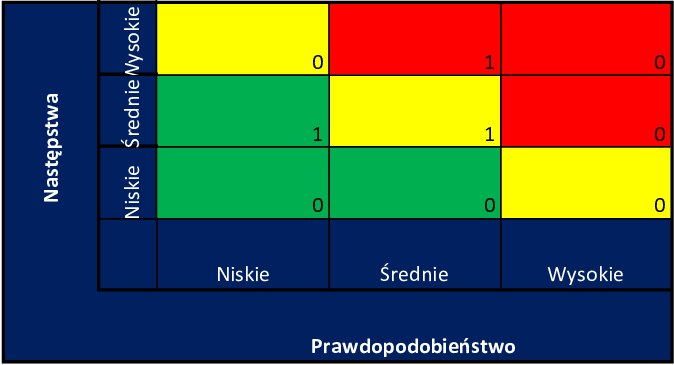
\includegraphics[width=.5\linewidth]{macierz_ryzyka.png}
	\caption{Macierz ryzyka}
\end{figure}

Macierz ryzyka tworzymy w celu określenia poziomu ryzyka związanego z~produkcją i~działaniem produktu w celu obniżenia negatywnego wpływu ryzyka na~funkcjonowanie danego podmiotu i~podejmowanie odpowiednich działań służących przeciwdziałaniu i~ograniczaniu ryzyka. Po~stworzeniu listy ryzyk i~oszacowaniu ryzyka dla każdego elementu z~listy można wywnioskować, że~najwyższe ryzyko jest związane z~błędem ludzkim (programisty). Minimalizować to~ryzyko możemy, testując oprogramowanie przed wdrożeniem oraz dbać o~obecność backupów na~wypadek problemów z~aktualizacją.

\begin{figure}[H]
	\centering
	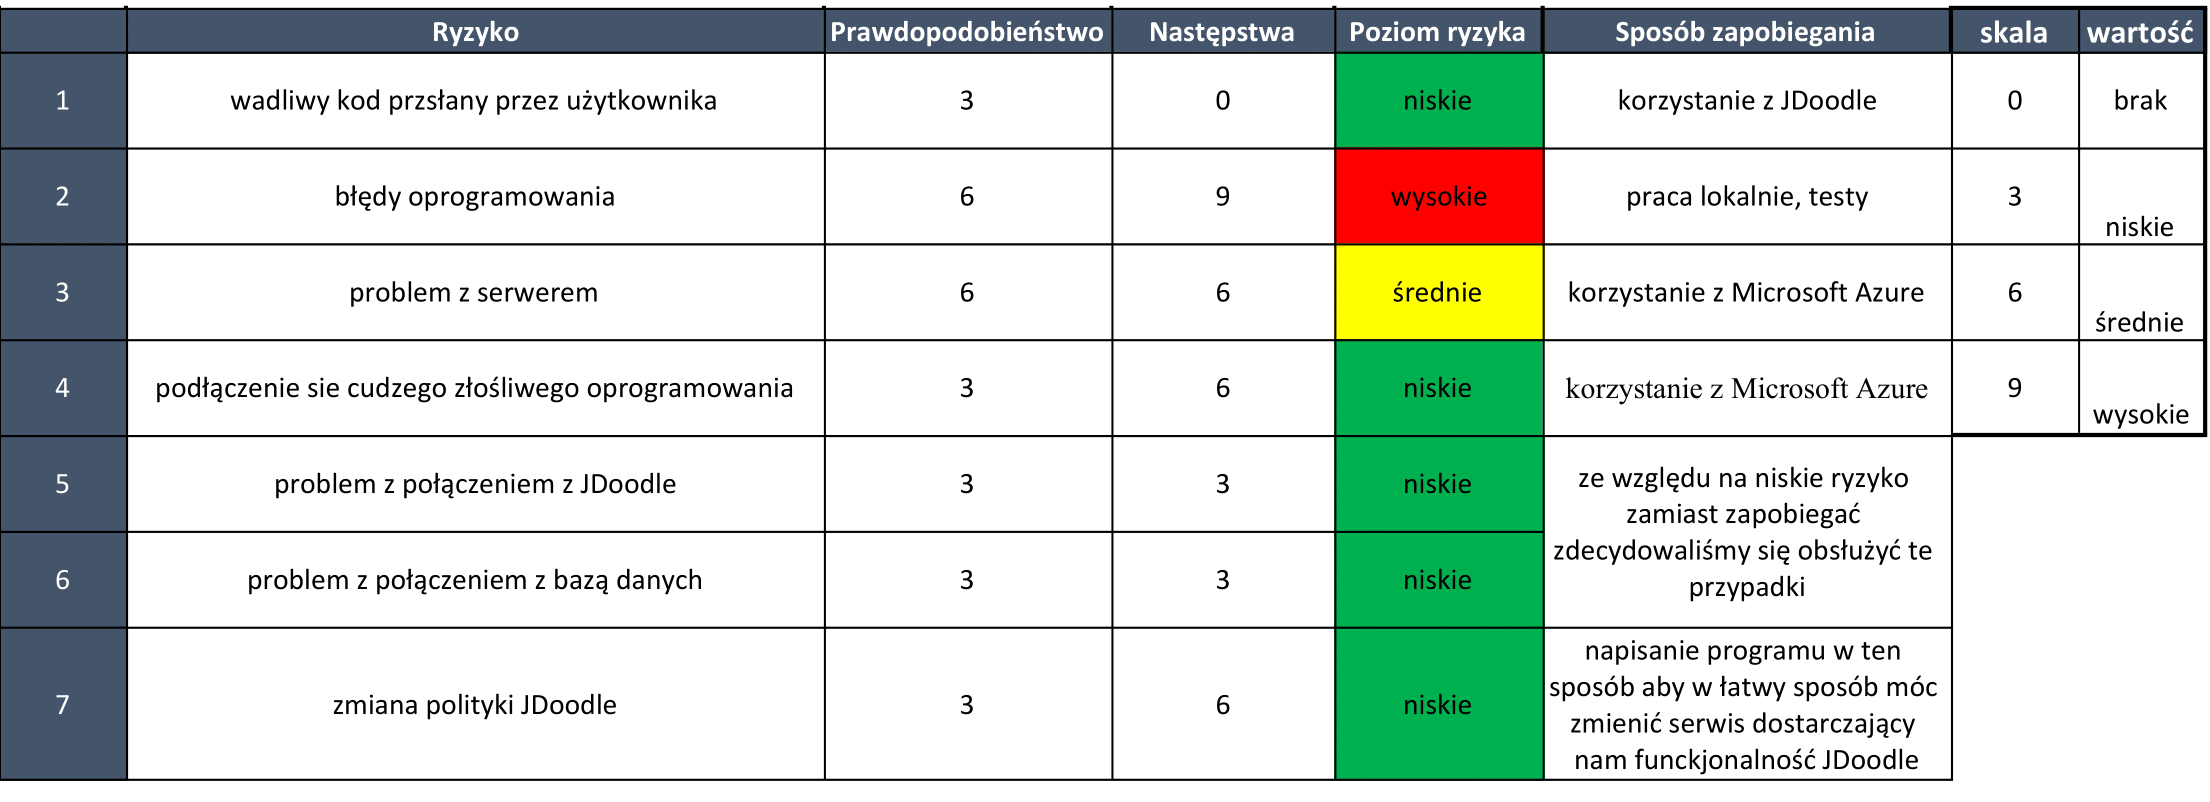
\includegraphics[width=.95\linewidth]{lista_ryzyk.png}
	\caption{Lista ryzyk}
\end{figure}

\end{document}
